\documentclass[11pt]{article}
\usepackage{geometry,marginnote} % Pour passer au format A4
\geometry{hmargin=1cm, vmargin=1.5cm} % 

% Page et encodage
\usepackage[T1]{fontenc} % Use 8-bit encoding that has 256 glyphs
\usepackage[english,french]{babel} % Français et anglais
\usepackage[utf8]{inputenc} 

\usepackage{lmodern}
\usepackage[np]{numprint}
\setlength\parindent{0pt}

% Graphiques
\usepackage{graphicx,float,grffile}
\usepackage{tikz,pst-eucl,pst-plot,pstricks,pst-node,pstricks-add,pst-fun,pgfplots} 

% Maths et divers
\usepackage{amsmath,amsfonts,amssymb,amsthm,verbatim,scratch3}
\usepackage{multicol,enumitem,url,eurosym,gensymb,tabularx}

\DeclareUnicodeCharacter{20AC}{\euro}



% Sections
\usepackage{sectsty} % Allows customizing section commands
\allsectionsfont{\centering \normalfont\scshape}

% Tête et pied de page
\usepackage{fancyhdr} \pagestyle{fancy} \fancyhead{} \fancyfoot{}

%\fancyfoot[L]{Collège Faubert}
%\fancyfoot[C]{\thepage / 6}
%\fancyfoot[R]{Série Générale}

\renewcommand{\headrulewidth}{0pt} % Remove header underlines
%\renewcommand{\footrulewidth}{0pt} % Remove footer underlines

\newcommand{\horrule}[1]{\rule{\linewidth}{#1}} % Create horizontal rule command with 1 argument of height

\newcommand{\Pointilles}[1][3]{%
  \multido{}{#1}{\makebox[\linewidth]{\dotfill}\\[\parskip]
}}

\newtheorem{Definition}{Définition}

\usepackage{siunitx}
\sisetup{
    detect-all,
    output-decimal-marker={,},
    group-minimum-digits = 3,
    group-separator={~},
    number-unit-separator={~},
    inter-unit-product={~}
}

\setlength{\columnseprule}{1pt}


\begin{document}

\section*{chap 1 - Pythagore}

\section*{1 - Le carré}

\begin{multicols}{2}

\subsection*{L'aire d'un carré}

  \begin{figure}[H]
    \centering
    \includegraphics[width=0.8\linewidth]{4x1-pythagore/fonction-carre.pdf}
  \end{figure}

\begin{itemize}
\item $Aire = c \times c = c^2$. 
\item $15^2 = 15 \times 15 = 225$
\end{itemize}

\subsection*{Le côté d'un carré}

  \begin{figure}[H]
    \centering
    \includegraphics[width=0.8\linewidth]{4x1-pythagore/fonction-racine.pdf}
  \end{figure}

\begin{itemize}
\item Il peut être difficile de retrouver le côté d'un carré quand on connaît son aire. 
\item $Aire = 25cm^2 \Rightarrow c = 5cm$ car $5 \times 5 = 25$ ;  $Aire = 16cm^2 \Rightarrow c = 4cm$ car $4 \times 4 = 16$.
\item $Aire = 20cm^2 \Rightarrow c = ?$
\end{itemize}

\end{multicols}

\section*{2 - Conjecture géométrique}

Dans un triangle rectangle, la somme des deux petits carrés est égale au grand carré.

  \begin{figure}[H]
    \centering
    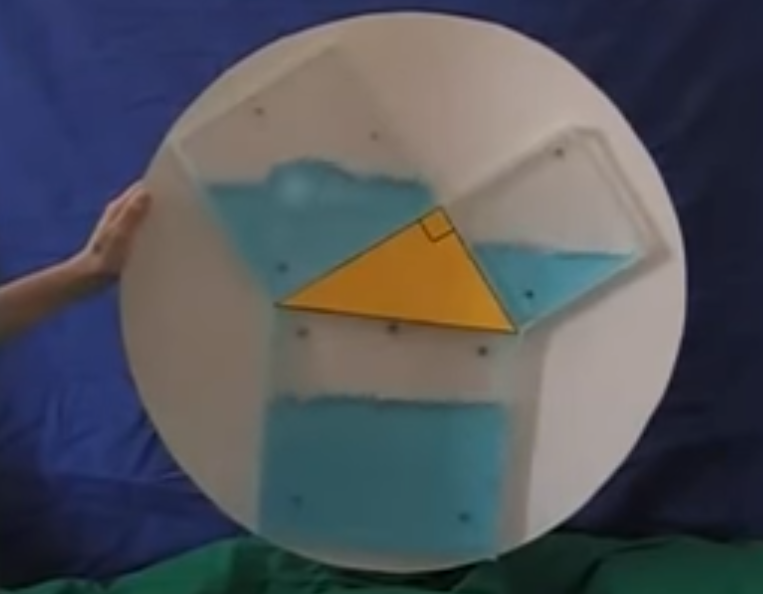
\includegraphics[width=0.4\linewidth]{4x1-pythagore/pyth.png}
  \end{figure}


\end{document}
